
\chapter{引言:\CTeX 系统的安装和使用}
\label{chap:introduction}

本模板(ustcthesis.cls)是按照教务处的本科论文要求做出的\LaTeX 模板,作者为XPS。\par
本文是使用上述模板生成的示例文档,目的在于帮助使用者熟悉该模板的使用方法,并且方便使用者学位论文的撰写。

\section{系统要求,\CTeX 安装}
本文只针对Windows环境下\CTeX 套装。至于Linux使用者,我觉得你们有能力解决自己的问题。\par
如果电脑上尚未安装\LaTeX 系统,那么到\href{http://www.ctex.org/}{CTeX.org}下载最新完整版\CTeX 套装,并安装之。\par
此模板只支持UTF-8编码。将其他编码的文件转化为UTF-8的方法是: 用记事本打开这些文件, 然后点击文件—另存为—在最下方选择UTF-8 编码。在WinEdt中首次保存时,选择save as...,弹出的窗口中保存类型选择:UTF-8即可。


\section{WinEdit界面介绍和使用}
\CTeX 套装试用WinEdt作为默认编辑器,什么都配置好了,很方便,推荐使用。

打开\CTeX 套装内的WinEdit编辑器,可以看到如图\ref{f:winedit}的界面。
\begin{figure}[ht]
\centering
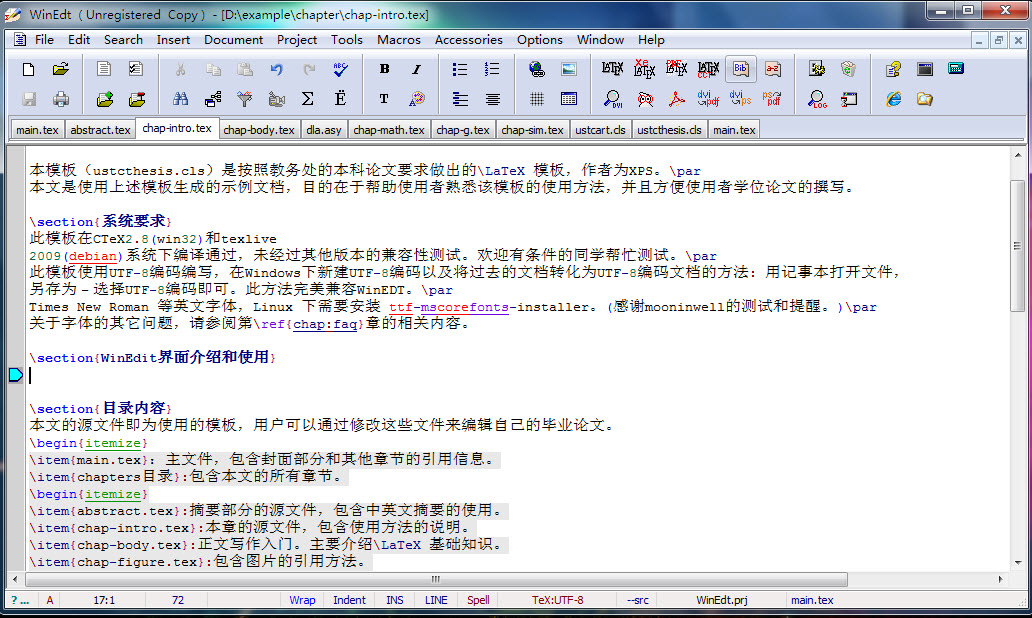
\includegraphics[width=0.8\textwidth]{winedit.jpg}
\caption{WinEdt界面}
\label{f:winedit}
\end{figure}

其中,中部的大块白色背景的区域就是键入文章内容的编辑区。编辑区上方的一条工具栏上有所有当前打开的文件的标签,单击即可跳转到对应文件。标签栏上方是面板,上面有一些很常用的工具按钮,鼠标悬停可以看到按钮名称。下面我们来看其中的几个。在使用本模板时,将会用到这些按钮。
\begin{itemize}
\item 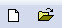
\includegraphics{open.jpg}\\
新建和打开按钮。
\item 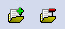
\includegraphics{mainfile.jpg}\\
单击左侧的按钮可设置主文件,单击右侧的取消主文件。
\item 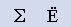
\includegraphics{mathhelp.jpg}\\
单击可以分别打开TeX SYMBOLS GUI(用于输入数学公式)和ASCII字符表。
\item 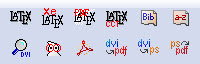
\includegraphics{compile.jpg}\\
编译区,我们需要使用的是上排第二个,第五个和下排第三个,即\XeLaTeX ,BibTeX和 Reader。
\end{itemize}

一般的写作流程是:准备好要写的文字和要插入的图片------在编辑区内输入文字------用各种\LaTeX 命令控制文章格式(第\ref{c:main}章),插入数学公式(第\ref{chap:math}章)、表格(第\ref{chap:tab}章)、图片(第\ref{chap:fig}章)等------编译(\ref{s:compile})------查看结果------修改,再编译------满意的文章。


\section{编译和调试方法}
\label{s:compile}
本模板需要使用\XeLaTeX 编译,切换到main.tex,点击面板上对应的按钮即可。如果你觉得每次都切过来很浪费时间,那么可以换到main.tex,并单击WinEdit工具栏上Set Main File按钮。这样的话以后每次编译都自动从main.tex开始,可以省掉不少麻烦。

如果编译出错,即停在某一位置不动了,且有问号提示符让使用者输入的话,那么按e回车,可以自动跳转到出错位置进行查看。出错的种类五花八门无法一一列举,但是一般都有详细的提示,如果有实在没法修正的可以到BBS TeX板提问。

编译通过之后,可以点工具栏上的Adobe按钮,打开预览。在CTeX2.8套装的WinEdit中,会弹出SumatraPDF,在这个窗口中,看到不合意的地方可以双击回到源文件的相应位置,逆向搜索到原文中的对应位置进行修改,还是比较方便的。\par

\begin{example}{Hello World}\\
将以下内容复制到新文件中,保存为\TeX 文件,编译,然后按Adobe按钮预览结果。
\begin{code}
    \documentclass{article}
    \begin{document}
        Hello world!
    \end{document}
\end{code}
\end{example}


为了得到正确的目录、交叉引用、参考文献等信息,需要编译两到三遍,正确的流程如下:
\begin{enumerate}
\item \XeLaTeX 编译一次。
\item BibTex编译一次。
\item \XeLaTeX 编译两到三次。
\end{enumerate}
在本示例文档中,提供了make.bat,双击之即可完成以上工作。



\section{目录内容}
本文的源文件即为使用的模板,用户可以通过修改这些文件来编辑自己的毕业论文。
\begin{itemize}
\item{main.tex}:主文件,包含封面部分和其他章节的引用信息。
\item{chapters目录}:包含本文的所有章节。
\begin{itemize}
\item{abstract.tex}:摘要部分的源文件,包含中英文摘要的使用。
\item{chap-intro.tex}:本章的源文件,包含使用方法的说明。
\item{chap-body.tex}:正文写作入门。主要介绍\LaTeX 基础知识。
\item{chap-figure.tex}:包含图片的引用方法。
\item{chap-table.tex}:包含表格的示例。
\item{chap-math.tex}:包含数学公式排版的基础知识。
\item{chap-app.tex}:附录。
\item{thanks.tex}包含致谢部分。
\end{itemize}
\item{figures目录}:存放文章内所用的图像文件。
\item{bib/tex.bib}:参考文献信息。
\end{itemize}
需要特别说明的是,这些文件名并不是固定的,你可以新建一个tex文件,例如zhangsan.tex,放在chapters目录下,并且在main.tex中使用
\begin{code}
    \include{chapters/zhangsan.tex}
\end{code}
来引用之。当然你也可以重命名这些文件,只要include中的文件名是存在的,\LaTeX 总能找到这些文件的。

在你写作某一章节的时候,你可能需要随时预览排版效果并debug,这时你可以在其他章节的\verb|\include|命令前加上一个\%,这代表注释掉本行,例如:
\begin{code}
    %%%%%%%%%%%%%%%%%%%%%%%%%%%%%%
    %% 正文部分
    %%%%%%%%%%%%%%%%%%%%%%%%%%%%%%
    \mainmatter
      
\chapter{绪论}
\label{chap:introduction}

中国科学技术大学,中国科学技术大学,中国科学技术大学,中国科学技术大学,中国科学技术大学,中国科学技术大学
中国科学技术大学,中国科学技术大学,中国科学技术大学


中国科学技术大学

\section{系统要求}



\section{下载与安装}


\href{http://code.google.com/p/ustcthesis}{http://code.google.com/p/ustcthesis}




\section{问题反馈}

用户在使用中遇到问题或者需要增加某种功能,请到\href{http://bbs.ustc.edu.cn/cgi/go?cgi=bbsdoc&board=TeX}{瀚海星云bbs,Tex版}反映。


欢迎大家反馈自己的使用情况,使我们可以不断改进宏包。

\section{为人民服务}


我们的共产党和共产党所领导的八路军、新四军,是革命的队伍。我们这个队伍完全是为着解放人民的,是彻底地为人民的利益工作的。张思德同志就是我们这个队伍中的一个同志。

人总是要死的,但死的意义有不同。中国古时候有个文学家叫做司马迁的说过:人固有一死,或重于泰山,或轻于鸿毛。为人民利益而死,就比泰山还重;替法西斯卖力,替剥削人民和压迫人民的人去死,就比鸿毛还轻。张思德同志是为人民利益而死的,他的死是比泰山还要重的。因为我们是为人民服务的,所以,我们如果有缺点,就不怕别人批评指出。不管是什么人,谁向我们指出都行。只要你说得对,我们就改正。你说的办法对人民有好处,我们就照你的办。“精兵简政”这一条意见,就是党外人士李鼎铭⑶先生提出来的;他提得好,对人民有好处,我们就采用了。只要我们为人民的利益坚持好的,为人民的利益改正错的,我们这个队伍就一定会兴旺起来。

我们都是来自五湖四海,为了一个共同的革命目标,走到一起来了。我们还要和全国大多数人民走这一条路。我们今天已经领导着有九千一百万人口的根据地,但是还不够,还要更大些,才能取得全民族的解放。我们的同志在困难的时候,要看到成绩,要看到光明,要提高我们的勇气。中国人民正在受难,我们有责任解救他们,我们要努力奋斗。要奋斗就会有牺牲,死人的事是经常发生的。但是我们想到人民的利益,想到大多数人民的痛苦,我们为人民而死,就是死得其所。不过,我们应当尽量地减少那些不必要的牺牲。我们的干部要关心每一个战士,一切革命队伍的人都要互相关心,互相爱护,互相帮助。

今后我们的队伍里,不管死了谁,不管是炊事员,是战士,只要他是做过一些有益的工作的,我们都要给他送葬,开追悼会。这要成为一个制度。这个方法也要介绍到老百姓那里去。村上的人死了,开个追悼会。用这样的方法,寄托我们的哀思,使整个人民团结起来。
    %  
\chapter{图形}
\label{chap:fig}


\section{浮动图形}

\XeLaTeX 支持jpg和eps格式的图片。我们所用的编译方法支持jpg和eps等格式的图片。如果你已经有一篇word文档,
想把其中的图全部导出,那么可以将它另存为html文件,这时会在同目录下找到一个文件夹,里面是所有用到的图片。

将插图放在figures文件夹中,想要引用的地方使用类似这样的命令插入图形文件:
\begin{code}
\begin{figure}[!ht]
 \centering
 
\includegraphics[width=0.2\textwidth]{ustc_logo_new.eps}
 \caption{中国科学技术大学校徽(在页面中间)}
 \label{fig:ustc1}
\end{figure}
\end{code}
结果如下:
\begin{figure}[!ht]
 \centering
 
\includegraphics[width=0.2\textwidth]{ustc_logo_new.eps}
 \caption{中国科学技术大学校徽(在页面中间)}
 \label{fig:ustc1}
\end{figure}

在上面这段命令中,可选参数[!ht]代表插图的位置。其中!让\LaTeX{}忽略审美标准,试图用最严格的标准来放置浮动图形;h(ere)代表有限放在此处;t(op)代表如果此处放不下,那么放在下一页页首。

width=0.2\textbackslash{}textwidth代表图形的宽度是文字宽度的0.2倍,你也可以使用其他长度单位,如12cm,4.5in等等。

caption命令的参数代表图的名称,或者说注解。label的参数用于交叉引用,见下节。


\section{交叉引用}
通过使用交叉引用功能,我们可以定位那些\LaTeX{}自动编号的内容,比如浮动图形、表格、章节等等。其中,label和ref的参数是引用的名字,可以随意,但须保持一致。
\begin{figure}[ht]
\centering
\fbox{\begin{minipage}[h]{0.4\textwidth}
引用图\ref{fig:ustc1}\\
引用第\ref{chap:introduction}章
\end{minipage}}
\hspace{0.1\textwidth}
\begin{minipage}[h]{0.4\textwidth}
\centering
\begin{code}
引用图\ref{fig:ustc1}\\
引用第\ref{chap:introduction}章
\end{code}
\end{minipage}
\caption{交叉引用示例}
\end{figure}


\section{并列的子图}
使用subfigure命令,一个例子:
\begin{figure}[!hbt]
\centering
\subfigure[sf 1]{

\includegraphics[width=0.2\textwidth]{ustc_logo_new.eps}\label{f:1}}
\subfigure[sf 2]{

\includegraphics[width=0.2\textwidth]{ustc_logo_new.eps}\label{f:2}}
\subfigure[sf 3]{

\includegraphics[width=0.2\textwidth]{ustc_logo_new.eps}\label{f:3}}
\subfigure[sf 4]{

\includegraphics[width=0.2\textwidth]{ustc_logo_new.eps}\label{f:4}}
\caption{\label{f:s}subfigure使用示例。}
\end{figure}
\begin{code}
\begin{figure}[!hbt]
\centering
\subfigure[sf 1]{

\includegraphics[width=0.2\textwidth]{ustc_logo_new.eps}\label{f:1}}
\subfigure[sf 2]{

\includegraphics[width=0.2\textwidth]{ustc_logo_new.eps}\label{f:2}}
\subfigure[sf 3]{

\includegraphics[width=0.2\textwidth]{ustc_logo_new.eps}\label{f:3}}
\subfigure[sf 4]{

\includegraphics[width=0.2\textwidth]{ustc_logo_new.eps}\label{f:4}}
\caption{\label{f:s}subfigure使用示例。}
\end{figure}
\end{code}

分两行放:
\begin{figure}[!hbt]
\centering
\subfigure[sf 1]{

\includegraphics[width=0.2\textwidth]{ustc_logo_new.eps}\label{f:1}}
\subfigure[sf 2]{

\includegraphics[width=0.2\textwidth]{ustc_logo_new.eps}\label{f:2}}\\
\subfigure[sf 3]{

\includegraphics[width=0.2\textwidth]{ustc_logo_new.eps}\label{f:3}}
\subfigure[sf 4]{

\includegraphics[width=0.2\textwidth]{ustc_logo_new.eps}\label{f:4}}
\caption{\label{f:s}subfigure使用示例。}
\end{figure}
\begin{code}
\begin{figure}[!hbt]
\centering
\subfigure[f 1]{

\includegraphics[width=0.2\textwidth]{ustc_logo_new.eps}\label{f:1}}
\subfigure[f 2]{

\includegraphics[width=0.2\textwidth]{ustc_logo_new.eps}\label{f:2}}\\
\subfigure[f 3]{

\includegraphics[width=0.2\textwidth]{ustc_logo_new.eps}\label{f:3}}
\subfigure[f 4]{

\includegraphics[width=0.2\textwidth]{ustc_logo_new.eps}\label{f:4}}
\caption{\label{f:l}分行的字图使用示例。}
\end{figure}
\end{code}
    %  
\chapter{表格}
\label{chap:tab}
标准三线表:
\begin{table}[!ht]
\label{tab:table3}
\caption{三线表格示例}
\centering
\begin{tabular}{c c c c}
\whline 一列 & 两列 & 三列 & 四列  \\\hline
1 & 2 &3 &4 \\2 & 3 &4 &5 \\3 & 4 &5 &6 \\
\whline
\end{tabular}
\end{table}
\begin{code}
    \begin{table}[!ht]
    \label{tab:table3}
    \caption{三线表格示例}
    \centering
    \begin{tabular}{c c c c}
        \whline 一列 & 两列 & 三列 & 四列  \\\whline
        1 & 2 &3 &4 \\2 & 3 &4 &5 \\3 & 4 &5 &6 \\
        \whline
    \end{tabular}
    \end{table}
\end{code}

与figure一样,table环境也是浮动体,常用!ht来表明位置。caption、label的意义都与figure环境相同。

而画表格的tabular环境则与array环境几乎相同,只是在每行之间可以用\textbackslash{}hline和\textbackslash{}hline这些命令来画横线。c代表一个居中对齐的列,l代表靠左对齐,r代表靠右对齐。
有竖线的例子:
\begin{table}[!ht]
\label{tab:table2}
\caption{表格示例2}
\centering
\begin{tabular}{ Ic|c|c|cI}
\whline 一列 & 两列 & 三列 & 四列  \\\hline
1 & 2 &3 &4 \\\hline 2 & 3 &4 &5 \\\hline3 & 4 &5 &6 \\
\whline
\end{tabular}
\end{table}
\begin{code}
    \begin{table}[!ht]
    \label{tab:table2}
    \caption{表格示例2}
    \centering
    \begin{tabular}{ Ic|c|c|cI}
        \whline 一列 & 两列 & 三列 & 四列  \\\hline
        1 & 2 &3 &4 \\\hline 2 & 3 &4 &5 \\\hline3 & 4 &5 &6 \\
        \whline
    \end{tabular}
    \end{table}
\end{code}

即竖线是|,粗竖线是大写字母I,横线是\textbackslash hline,粗横线是\textbackslash whline。

    %  
\chapter{数学公式}
\label{chap:math}
\begin{equation}
\begin{split}
\mbox{Pr}\{S_i=0\}=\frac{a_i}{b_i+a_i} \\
\mbox{Pr}\{S_i=1\}=\frac{b_i}{b_i+a_i} \label{1}
\end{split}
\end{equation}\cite{lshort-cn}



\begin{table}[htbp]
\centering
\caption{基于因子分析的失配补偿结果}\label{tab:jfa-gmm-ubm}
\begin{tabular}{cccccc}
    \toprule
    &\multirow{2}{*}{\#Mix}&\multicolumn{2}{c}{No-norm}
    &\multicolumn{2}{c}{Tnorm}\\
    \cline{3-4} \cline{5-6}
		&		& EER(\%) 	& MinDCF & EER(\%) 	& MinDCF\\
    \midrule
	\multirow{3}{*}{GMM-UBM}
    &256 		& 12.43 	& 0.0647	& 12.85    & 0.0580\\
    &512 		& 10.02 	& 0.0464	& 8.88 	   & 0.0370\\
    &1024 		& 9.97 	    & 0.0457	& 8.72 	   & 0.0372\\
    \midrule
	\multirow{3}{*}{Factor Analysis}
    &256 		& 8.09 	& 0.0331 	& 7.39 	& 0.0319\\
    &512 		& 7.08 	& 0.0305 	& 6.53 	& 0.0292\\
    &1024 		& 6.83 	& 0.0295 	& \textbf{6.29} 	& \textbf{0.0279}\\
 \bottomrule
\end{tabular}
\end{table}



\IncMargin{1em}
\begin{algorithm}
\SetKwData{Left}{left}\SetKwData{This}{this}\SetKwData{Up}{up}
\SetKwFunction{Union}{Union}\SetKwFunction{FindCompress}{FindCompress}
\SetKwInOut{Input}{input}\SetKwInOut{Output}{output}
\Input{$O_t,UBM,U$}
\Output{$x,y$}
\BlankLine
\emph{$y\leftarrow 0;$$x_h\leftarrow 0;$$h=1,...,H$ }\;
\For{$i=1$ \KwTo Number of E-M iterations}{
\emph{E Step}:\\
\For{$h=1$ \KwTo $H$}{\label{forins}
对于每一条语音段,计算其EM统计量(零阶统计量$N_h$,一阶统计量$S_{X,h}$\;
}
计算每一个人所有语音段的零阶统计量$N$\\
计算每一个人所有语音段的一阶统计量$S$\\
\emph{M Step}:\\
\For{$j=1$ \KwTo Number of Gauss-Seidel iterations}{
\For{$h=1$ \KwTo $H$}{\label{forins}
估计每一语音段$h$的失配因子$x_h$
}
估计模型的话者因子$y$
}
}
\Return{$\mu = m+Dy$}
\caption{disjoint decomposition}\label{algo_disjdecomp}
\end{algorithm}\DecMargin{1em}
    %  
\chapter{常见问题}
\label{chap:faq}

\newtheoremstyle{question}% name
  {}%      Space above, empty = `usual value'
  {}%      Space below
  {\tt}% Body font
  {}%         Indent amount (empty = no indent, \parindent = para indent)
  {\bfseries}% Thm head font
  {.}%        Punctuation after thm head
  {10pt}% Space after thm head: \newline = linebreak
  {}%         Thm head spec

\newtheoremstyle{answer}% name
  {}%      Space above, empty = `usual value'
  {}%      Space below
  {\rm}% Body font
  {}%         Indent amount (empty = no indent, \parindent = para indent)
  {\bfseries}% Thm head font
  {.}%        Punctuation after thm head
  {10pt}% Space after thm head: \newline = linebreak
  {}%         Thm head spec

\theoremstyle{question}
 \newtheorem{FAQ}{问题~}
\theoremstyle{answer}
 \newtheorem{ANS}{回答~}

\section{表格}

\begin{FAQ}
页眉里论文题目和各章标题中的字母均为大写,不能实现大小写的区别,而我写的论文需要在页眉中出现的标题中区分英文字母的大小写比如:YBaCuO而不是YBACUO。
\end{FAQ}

\begin{ANS}
在 CASthesis.cfg 文件中加上
\begin{verbatim}
\renewcommand\title[2][\CAST@value@title]{%
  \def\CAST@value@title{#2}
  \def\CAST@value@titlemark{#1}}
\def\chaptermark#1{\markboth {{\ifnum \c@secnumdepth>\m@ne
  \if@mainmatter\CTEXthechapter \quad\fi
  \fi #1}}{}}%
\def\sectionmark#1{\markright{{\ifnum \c@secnumdepth >\z@
  \CTEXthesection \quad \fi #1}}}
\end{verbatim}
\end{ANS}


\section{脚注}

\begin{FAQ}
如果在章节标题中加入注脚,则不仅会出现在本章首页的页脚,也会出现在目录的页脚,不知是否能够让其不要出现在目录的页脚中。
\end{FAQ}

\begin{ANS}
可以使用如下的命令来定义章节的标题
\begin{verbatim}
\chapter[出现在目录和页眉的标题]{出现在正文的标题\footnote{这个不会出现在目录中。}}
\end{verbatim}
section、~subsection 等命令也有类似的用法。
\end{ANS}

\end{code}
那么,编译的时候就只编译未加\%的一章,在这个例子中,即本章。

理论上,并不一定要把每章放在不同的文件中,但是这种分章节写作、编译的方法有利于提高效率,大大减少debug过程中的编译时间,同时减小风险。 